\documentclass[a4paper,11pt,notitlepage]{report}

\usepackage{graphicx}
\usepackage[utf8]{inputenc}
\usepackage[T1]{fontenc}
\usepackage[ngerman]{babel}
\usepackage{bibgerm}
\usepackage{amsmath,amssymb,amsthm}
\usepackage{color}
\usepackage{enumerate}
\usepackage{tabularx}
\usepackage{subfig}
\usepackage{fancyhdr}
\usepackage{upgreek}
\usepackage[pdftex,pdfpagelabels,colorlinks,backref,pagebackref]{hyperref}
\usepackage{tikz} % SELBST HINZUGEFÜGT
\usepackage{lmodern}
% == Set the heading style ===================================================
\setlength{\headheight}{14pt}
\pagestyle{fancyplain}
\renewcommand{\chaptermark}[1]{\markboth{#1}{}}
\renewcommand{\sectionmark}[1]{\markright{\thesection\ #1}}
\lhead[\fancyplain{}{\thepage}]{\fancyplain{}{\rightmark}}
\rhead[\fancyplain{}{\leftmark}]{\fancyplain{}{\thepage}}
\cfoot{}
\renewcommand{\headrulewidth}{0.4pt}
% ============================================================================

% == Set correct values for fitting floats ===================================
\tolerance=2000
\emergencystretch=10pt

\setcounter{topnumber}{3}
\setcounter{totalnumber}{5}
\setcounter{bottomnumber}{2}

% To make those darn floats fit where they should
\setcounter{totalnumber}{9}
\setcounter{topnumber}{9}
\setcounter{bottomnumber}{9}
\renewcommand{\textfraction}{0.00}
\renewcommand{\topfraction}{1.0}
\renewcommand{\bottomfraction}{1.0}
% ============================================================================

% == German definitions for theorems etc. ==================================== 
\newtheorem{definition}{Definition}[chapter]
\newtheorem{theorem}{Satz}[chapter]
\newtheorem{lemma}{Lemma}[chapter]
\newtheorem{proposition}{Proposition}[chapter]
\newtheorem{corollary}{Korollar}[chapter]
\newtheorem{observation}{Beobachtung}[chapter]
\newtheorem{fact}{Fakt}[chapter]
\newtheorem{remark}{Bemerkung}[chapter]
\newtheorem{example}{Beispiel}[chapter]
% ============================================================================

% == Abkürzungen für die reellen, natürlichen, ganzen,... Zahlen =============
\newcommand{\R}{{\ensuremath{\mathbb{R}}}}
\newcommand{\N}{{\ensuremath{\mathbb{N}}}}
\newcommand{\Z}{{\ensuremath{\mathbb{Z}}}}
\newcommand{\C}{{\ensuremath{\mathbb{C}}}}
\newcommand{\Q}{{\ensuremath{\mathbb{Q}}}}
\newcommand{\F}{{\ensuremath{\mathbb{F}}}}
\newcommand{\Prim}{{\ensuremath{\mathbb{P}}}}
% ============================================================================

% == Makros für Autorenname und -adresse =====================================
\newcommand{\myaddress}[6]{%
  \parbox{\textwidth}{\textbf{\large #1}\\
    #2\\ #3\\ #4\\ 
    \ifthenelse{\equal{#5}{}}{}{Email: \href{mailto:#5}{\texttt{#5}}\\}
    \ifthenelse{\equal{#6}{}}{}{WWW: \href{#6}{\path|#6|}\\}
  } 
}

\newcommand{\myauthor}[1]{%
  \addtocontents{toc}{\protect\hspace{3.35ex}%
  \textsl{#1}\par}\vspace{-4ex}\quad\hfill\textsl{\Large #1}\vspace{8ex}}

\newcommand{\myname}[1]{\Large #1}

\title{\textbf{{Einführung in die Geometrie und Topologie - Mitschrieb -} \\[5ex] 
    {\Large Übung im Wintersemester 2011/2012\\[5ex]}}}

%%%%%%%%%%%%%%%%%%%%%%%%%%%%%%%%%%%%%%%%%%%%%%%%%%
% Tragen Sie in der folg. Zeile Ihren Namen ein: %
%%%%%%%%%%%%%%%%%%%%%%%%%%%%%%%%%%%%%%%%%%%%%%%%%%
\author{\myname{Sarah Lutteropp}}


\newcommand{\OO}{{\ensuremath{\mathcal{O}}}}

\begin{document}
\shorthandoff{"}
\begin{titlepage}
	\begin{center}	
		\LARGE \textbf{{Einführung in die Geometrie und Topologie - Mitschrieb -} \\[5ex] 
    		{\Large Übung im Wintersemester 2011/2012\\[5ex]}}
	\end{center}
	\begin{center}
		\Large Sarah Lutteropp
	\end{center}
	\begin{center}
		\today
	\end{center}
	\vspace{2cm}
	\begin{center}
		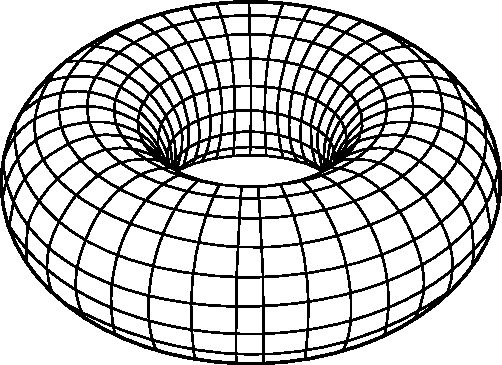
\includegraphics[width=0.8\textwidth]{torus2.pdf}
	\end{center}
\end{titlepage}
%\maketitle
\setcounter{tocdepth}{1}
\tableofcontents

\section*{Vorwort}
Dies ist ein Mitschrieb der Übung “Einführung in die Geometrie und Topologie” vom Wintersemester 2011/2012 am Karlsruher Institut für Technologie, die von Frau Dipl.-Math. Sandra Lenz gehalten wird.

\chapter{24.10.2011}

\begin{section}{Induzierte Topologie}
	\begin{definition}[Induzierte Topologie]
		Sei $X$ eine Menge. Sei $d \colon X \times X \rightarrow \R$ eine Metrik. Diese Metrik $d$ definiert durch folgende Bedingung eine Topologie $\OO$ auf $X$:
		\newline
		$O \subseteq X$ ist genau dann offen (d.h. $O \in \OO_d$), wenn für alle $x \in O$ ein $\epsilon > 0$ existiert mit
		$$
			B_\epsilon (x) := \{y \in X \mid d(x,y) < \epsilon\} \subseteq O.
		$$
		($B_\epsilon$ nennt man offenen $\epsilon$-Ball.)
	\end{definition}
\end{section}

\begin{section}{Offen und abgeschlossen}
	Sei $X$ eine Menge.
	\begin{itemize}
		\item Mengen können sowohl offen als auch abgeschlossen (zugleich) sein.
			\begin{example}
				Betrachte $\emptyset$ und $X$ in der trivialen Topologie $\OO = \{X, \emptyset\}$.
					\newline
					Es gilt: $X \in \OO, \emptyset \in \OO$ nach Definition, d.h. $X$ und $\emptyset$ sind offen.
					\newline
					Außerdem gilt: $X^c = \emptyset \in \OO$, ebenso: $\emptyset^c = X \in \OO$, d.h. die Komplemente von $X$ und $\emptyset$ sind offen und somit $X$ und $\emptyset$ abgeschlossen.
			\end{example}
			
		\item Mengen können weder offen noch abgeschlossen sein.
			\begin{example}
				Betrachte $\R$ mit der von der Standardmetrik induzierten Topologie. Es ist $[0,1[$ nicht offen in dieser Topologie, denn für den Punkt $0$ finden wir kein $\epsilon > 0$, so dass $B_\epsilon(0)$ in $[0,1[$ liegt.
				Die Menge $[0,1[$ ist aber auch nicht abgeschlossen, da ihr Komplement $\R \backslash [0,1[ = ]-\infty,0[ \cup [\underline{1},\infty[$ nicht offen ist.
			\end{example}
		\item Bilder offener Mengen unter stetigen Abbildungen müssen nicht notwendigerweise offen sein.
			\begin{example}
				Betrachte $\R$ mit der von der Standardmetrik induzierten Topologie.
				\newline
				Definiere $f \colon \R \rightarrow \R, x \mapsto x^2$.
				\newline
				Es gilt für die in $\R$ offene Menge $]-1,1[$:
				\newline
				$f(]-1,1[)=[0,1[$ und $[0,1[$ ist nicht offen in $\R$.
			\end{example}
	\end{itemize}
\end{section}

\begin{section}{Basis der von der Standardmetrik auf dem $\R^n$ definierten Topologie}
	$$\mathcal{B} = \{B_{\frac{1}{m}}(x) \mid x \in \Q^n, m \in \N\}$$
	Diese Basis ist abzählbar.
\end{section}

\begin{section}{Teilraumtopologie}
	Es sei $(X, \OO)$ ein topologischer Raum, $A \subseteq X$.
	\newline
	Die Teilraumtopologie (oder Spurtopologie) ist definiert durch
	$$\OO \big |_{A} := \{U \cap A \mid U \in \OO\} $$
	
	\begin{theorem}
		In der Tat definiert $\OO \big |_{A}$ eine Topologie auf $A$.
	\end{theorem}
	
	\begin{proof}
			$\bullet$\underline{z.z.}: Für jede Indexmenge $I$ gilt:
				$\forall i \in I \colon O_i \in \OO \big |_{A} \Rightarrow \bigcup\limits_{i \in I}{O_i} \in \OO \big |_{A}.$
			\newline
			Sei $I$ beliebige Indexmenge. Für alle $i \in I$ mit $O_i \in \OO \big |_{A}$ gilt:
			Es existieren $\mathcal{U}_i \in \OO$ mit $O_i= \mathcal{U}_i \cap A$.
			Es gilt:
			$$\bigcup\limits_{i \in I}{O_i} = \bigcup\limits_{i \in I}{(\mathcal{U}_i \cap A) } = (\bigcup\limits_{i \in I}{\mathcal{U}_i})\cap A \in \OO \big |_{A}$$ (da $\bigcup\limits_{i \in I}{\mathcal{U}_i} \in \OO$).
			\newline
			$\bullet$ \underline{z.z.}: $\forall O_1, O_2 \in \OO \big |_{A} \colon O_1 \cap O_2 \in \OO \big |_{A}.$
			\newline
			Seien $O_1, O_2 \in \OO \big |_{A}$. Dann ex. $\mathcal{U}_1, \mathcal{U}_2 \in \OO$ mit $O_i = \mathcal{U}_i \cap A, i \in \{1,2\}.$ Es gilt:
			$O_1 \cap O_2 = (\mathcal{U}_1 \cap A) \cap (\mathcal{U}_2 \cap A) = (\mathcal{U}_1 \cap \mathcal{U}_2) \cap A \in \OO \big |_{A} \text{, da } \mathcal{U}_1 \cap \mathcal{U}_2 \in \OO.$
			\newline
			$\bullet$ \underline{z.z.}: $A, \emptyset \in \OO \big |_{A}.$
			\newline
			Es gilt: $A = X \cap A \in \OO \big |_{A}\text{, da } X \in \OO$ nach Definition von $\OO$. 
			\newline
			Es gilt: $\emptyset = \emptyset \cap A \in \OO \big |_{A} \text{, da } \emptyset \in \OO$ nach Definition von $\OO$.
	\end{proof}
\end{section}

\begin{section}{Homotopieäquivalenz}
	\begin{definition}
		Seien $X,Y$ topologische Räume. $X$ heißt \underline{homotopieäquivalent zu Y}, falls es stetige Abbildungen $f \colon X \rightarrow Y$ und $g \colon Y \rightarrow X$ gibt, so dass $f \circ g \simeq id_Y$ und $g \circ f \simeq id_X$.
	\end{definition}
	
	\begin{theorem}
		$\R^n \backslash \{0\}$ ist homotopieäquivalent zur Sphäre $S^{n-1}$.
	\end{theorem}
	
	\begin{proof}
		Sei $f \colon S^{n-1} \hookrightarrow \R^n \backslash \{0\}, x \mapsto x$ (Inklusionsabbildung). Dann ist $f$ stetig.
		\newline
		Sei weiter $g \colon \R^n \backslash \{0\} \rightarrow S^{n-1}, x \mapsto \frac{x}{||x||}$. Dann ist auch $g$ stetig und es gilt:
		$g \circ f = id_{S^{n-1}}$, also insbesondere $g \circ f \simeq id_{S^{n-1}}$.
		\newline
		Für $f \circ g$ betrachte folgende Abbildung:
		$$H \colon \R^n \backslash \{0\} \times [0,1] \rightarrow \R^n \backslash \{0\}, (x,t) \mapsto (1-t) \frac{x}{||x||} + t \cdot x$$
		Dann ist $H$ stetig und es gilt für alle $x \in \R \backslash \{0\}$:
		\newline
		$H(x,1) = x = id_{\R^n \backslash \{0\}}(x)$
		\newline
		$H(x,0) = \frac{x}{||x||} = (f \circ g)(x)$
		\newline
		Dann ist $H$ Homotopie von $f \circ g$ nach $id_{\R^n \backslash \{0\}}$ (in Zeichen: $f \circ g \simeq id_{\R^n \backslash \{0\}}$).
	\end{proof}
\end{section}
\end{document}
